\documentclass[11pt]{article}

% Shared notes settings for Applied Machine Learning lectures (UPES).
% Keep this file free of \documentclass to allow reuse via \input.

\usepackage[utf8]{inputenc}
\usepackage[T1]{fontenc}
\usepackage{lmodern}          % scalable T1 fonts; without this pdflatex falls back
\input{glyphtounicode}        % to bitmapped EC Type 3 and the PDFs are neither
\pdfgentounicode=1            % searchable nor screen-reader friendly
\usepackage[a4paper,margin=1in]{geometry}
\usepackage{hyperref}
\usepackage{xurl}
\usepackage{booktabs}
\usepackage{amsmath}
\usepackage{amssymb}
\usepackage{listings}
\usepackage{xcolor}
\usepackage{enumitem}
\usepackage{parskip}

% Code listings (Python-oriented for this subject).
\lstset{
  language=Python,
  basicstyle=\ttfamily\small,
  keywordstyle=\color{blue},
  commentstyle=\color{gray},
  stringstyle=\color{teal},
  showstringspaces=false,
  columns=fullflexible,
  frame=single,
  framerule=0.2pt,
  breaklines=true
}

\setlist[itemize]{topsep=0.3em,itemsep=0.2em}
\setlist[enumerate]{topsep=0.3em,itemsep=0.2em}

% Simple per-section source line.
\newcommand{\notesources}[1]{\par\noindent{\small\color{gray}\textit{Sources:} \sloppy #1\par}}

% Unit-wise source strings for this subject (used by slides + notes).
% Path is relative to the lecture `latex/` folder (the compilation CWD).
\IfFileExists{../../../_shared/aml-sources.tex}{%
  % Source strings for Applied Machine Learning (CSAI2017P) — used by slides + notes.
% Prescribed texts and reference books are taken from the course syllabus.
% Support texts are the author-hosted open-access editions:
%   statlearning.com            (ISL with Python)
%   probml.github.io/pml-book   (Murphy, Probabilistic Machine Learning)
%   d2l.ai                      (Dive into Deep Learning)
%   mml-book.github.io          (Mathematics for Machine Learning)

\newcommand{\AMLRepoURL}{https://github.com/tali7c/Applied-Machine-Learning}

% --- prescribed -------------------------------------------------------------
\newcommand{\AMLPrescribed}{%
M\"uller and Guido, \textit{Introduction to Machine Learning with Python}, O'Reilly, 2016.;%
Bishop, \textit{Pattern Recognition and Machine Learning}, Springer, 2006.;%
Murphy, \textit{Machine Learning: A Probabilistic Perspective}, MIT Press, 2012.;%
Han, Kamber and Pei, \textit{Data Mining: Concepts and Techniques} (3e), Morgan Kaufmann, 2012.%
}

% --- unit-wise ---------------------------------------------------------------
\newcommand{\AMLUnitISources}{%
M\"uller and Guido, \textit{Introduction to Machine Learning with Python}, Ch. 1.;%
Bishop, \textit{Pattern Recognition and Machine Learning}, Ch. 1.;%
Murphy, \textit{Probabilistic Machine Learning: An Introduction}, MIT Press, 2022, Ch. 1.;%
Mitchell, \textit{Machine Learning}, McGraw Hill, 1997, Ch. 1.;%
Scikit-learn documentation, accessed 2026-08-04.%
}

\newcommand{\AMLUnitIISources}{%
Bishop, \textit{Pattern Recognition and Machine Learning}, \S1.5, \S4.3, \S7.1.;%
Zhang, Lipton, Li and Smola, \textit{Dive into Deep Learning}, \S3.4.;%
Shalev-Shwartz and Ben-David, \textit{Understanding Machine Learning}, Ch. 15.;%
Murphy, \textit{Probabilistic Machine Learning: An Introduction}, Ch. 5.%
}

\newcommand{\AMLUnitIIISources}{%
Zhang, Lipton, Li and Smola, \textit{Dive into Deep Learning}, Ch. 12 (Optimization Algorithms).;%
Deisenroth, Faisal and Ong, \textit{Mathematics for Machine Learning}, Ch. 7.;%
Kingma and Ba, ``Adam: A Method for Stochastic Optimization,'' ICLR 2015.;%
Ruder, ``An overview of gradient descent optimization algorithms,'' arXiv:1609.04747, 2016.%
}

\newcommand{\AMLUnitIVSources}{%
Han, Kamber and Pei, \textit{Data Mining: Concepts and Techniques} (3e), Ch. 3.;%
M\"uller and Guido, \textit{Introduction to Machine Learning with Python}, Ch. 3--4.;%
James, Witten, Hastie, Tibshirani and Taylor, \textit{An Introduction to Statistical Learning with Python}, Ch. 5--6, 12.;%
Scikit-learn documentation (preprocessing, model selection), accessed 2026-08-04.%
}

\newcommand{\AMLUnitVSources}{%
James et al., \textit{An Introduction to Statistical Learning with Python}, Ch. 3--6.;%
Bishop, \textit{Pattern Recognition and Machine Learning}, Ch. 3.;%
Deisenroth, Faisal and Ong, \textit{Mathematics for Machine Learning}, Ch. 9.;%
M\"uller and Guido, \textit{Introduction to Machine Learning with Python}, \S2.3.%
}

\newcommand{\AMLUnitVISources}{%
Han, Kamber and Pei, \textit{Data Mining: Concepts and Techniques} (3e), Ch. 8--9.;%
James et al., \textit{An Introduction to Statistical Learning with Python}, Ch. 8--9.;%
Bishop, \textit{Pattern Recognition and Machine Learning}, Ch. 4--5, 7, 14.;%
Zhang et al., \textit{Dive into Deep Learning}, Ch. 5.%
}

\newcommand{\AMLUnitVIISources}{%
Han, Kamber and Pei, \textit{Data Mining: Concepts and Techniques} (3e), Ch. 10.;%
James et al., \textit{An Introduction to Statistical Learning with Python}, Ch. 12.;%
M\"uller and Guido, \textit{Introduction to Machine Learning with Python}, \S3.5.;%
Ester, Kriegel, Sander and Xu, ``A density-based algorithm for discovering clusters (DBSCAN),'' KDD 1996.%
}

\newcommand{\AMLLabSources}{%
M\"uller and Guido, \textit{Introduction to Machine Learning with Python}, companion notebooks.;%
McKinney, \textit{Python for Data Analysis} (3e), O'Reilly, 2022.;%
Scikit-learn user guide, accessed 2026-08-04.;%
Matplotlib and Seaborn documentation, accessed 2026-08-04.%
}
%
}{%
  % Faculty copies live under `private/` so their compile CWD is different.
  \IfFileExists{../../../../public/_shared/aml-sources.tex}{%
    % Source strings for Applied Machine Learning (CSAI2017P) — used by slides + notes.
% Prescribed texts and reference books are taken from the course syllabus.
% Support texts are the author-hosted open-access editions:
%   statlearning.com            (ISL with Python)
%   probml.github.io/pml-book   (Murphy, Probabilistic Machine Learning)
%   d2l.ai                      (Dive into Deep Learning)
%   mml-book.github.io          (Mathematics for Machine Learning)

\newcommand{\AMLRepoURL}{https://github.com/tali7c/Applied-Machine-Learning}

% --- prescribed -------------------------------------------------------------
\newcommand{\AMLPrescribed}{%
M\"uller and Guido, \textit{Introduction to Machine Learning with Python}, O'Reilly, 2016.;%
Bishop, \textit{Pattern Recognition and Machine Learning}, Springer, 2006.;%
Murphy, \textit{Machine Learning: A Probabilistic Perspective}, MIT Press, 2012.;%
Han, Kamber and Pei, \textit{Data Mining: Concepts and Techniques} (3e), Morgan Kaufmann, 2012.%
}

% --- unit-wise ---------------------------------------------------------------
\newcommand{\AMLUnitISources}{%
M\"uller and Guido, \textit{Introduction to Machine Learning with Python}, Ch. 1.;%
Bishop, \textit{Pattern Recognition and Machine Learning}, Ch. 1.;%
Murphy, \textit{Probabilistic Machine Learning: An Introduction}, MIT Press, 2022, Ch. 1.;%
Mitchell, \textit{Machine Learning}, McGraw Hill, 1997, Ch. 1.;%
Scikit-learn documentation, accessed 2026-08-04.%
}

\newcommand{\AMLUnitIISources}{%
Bishop, \textit{Pattern Recognition and Machine Learning}, \S1.5, \S4.3, \S7.1.;%
Zhang, Lipton, Li and Smola, \textit{Dive into Deep Learning}, \S3.4.;%
Shalev-Shwartz and Ben-David, \textit{Understanding Machine Learning}, Ch. 15.;%
Murphy, \textit{Probabilistic Machine Learning: An Introduction}, Ch. 5.%
}

\newcommand{\AMLUnitIIISources}{%
Zhang, Lipton, Li and Smola, \textit{Dive into Deep Learning}, Ch. 12 (Optimization Algorithms).;%
Deisenroth, Faisal and Ong, \textit{Mathematics for Machine Learning}, Ch. 7.;%
Kingma and Ba, ``Adam: A Method for Stochastic Optimization,'' ICLR 2015.;%
Ruder, ``An overview of gradient descent optimization algorithms,'' arXiv:1609.04747, 2016.%
}

\newcommand{\AMLUnitIVSources}{%
Han, Kamber and Pei, \textit{Data Mining: Concepts and Techniques} (3e), Ch. 3.;%
M\"uller and Guido, \textit{Introduction to Machine Learning with Python}, Ch. 3--4.;%
James, Witten, Hastie, Tibshirani and Taylor, \textit{An Introduction to Statistical Learning with Python}, Ch. 5--6, 12.;%
Scikit-learn documentation (preprocessing, model selection), accessed 2026-08-04.%
}

\newcommand{\AMLUnitVSources}{%
James et al., \textit{An Introduction to Statistical Learning with Python}, Ch. 3--6.;%
Bishop, \textit{Pattern Recognition and Machine Learning}, Ch. 3.;%
Deisenroth, Faisal and Ong, \textit{Mathematics for Machine Learning}, Ch. 9.;%
M\"uller and Guido, \textit{Introduction to Machine Learning with Python}, \S2.3.%
}

\newcommand{\AMLUnitVISources}{%
Han, Kamber and Pei, \textit{Data Mining: Concepts and Techniques} (3e), Ch. 8--9.;%
James et al., \textit{An Introduction to Statistical Learning with Python}, Ch. 8--9.;%
Bishop, \textit{Pattern Recognition and Machine Learning}, Ch. 4--5, 7, 14.;%
Zhang et al., \textit{Dive into Deep Learning}, Ch. 5.%
}

\newcommand{\AMLUnitVIISources}{%
Han, Kamber and Pei, \textit{Data Mining: Concepts and Techniques} (3e), Ch. 10.;%
James et al., \textit{An Introduction to Statistical Learning with Python}, Ch. 12.;%
M\"uller and Guido, \textit{Introduction to Machine Learning with Python}, \S3.5.;%
Ester, Kriegel, Sander and Xu, ``A density-based algorithm for discovering clusters (DBSCAN),'' KDD 1996.%
}

\newcommand{\AMLLabSources}{%
M\"uller and Guido, \textit{Introduction to Machine Learning with Python}, companion notebooks.;%
McKinney, \textit{Python for Data Analysis} (3e), O'Reilly, 2022.;%
Scikit-learn user guide, accessed 2026-08-04.;%
Matplotlib and Seaborn documentation, accessed 2026-08-04.%
}
%
  }{%
    % Question papers live at `private/<family>/<instrument>/`.
    \IfFileExists{../../../public/_shared/aml-sources.tex}{%
      % Source strings for Applied Machine Learning (CSAI2017P) — used by slides + notes.
% Prescribed texts and reference books are taken from the course syllabus.
% Support texts are the author-hosted open-access editions:
%   statlearning.com            (ISL with Python)
%   probml.github.io/pml-book   (Murphy, Probabilistic Machine Learning)
%   d2l.ai                      (Dive into Deep Learning)
%   mml-book.github.io          (Mathematics for Machine Learning)

\newcommand{\AMLRepoURL}{https://github.com/tali7c/Applied-Machine-Learning}

% --- prescribed -------------------------------------------------------------
\newcommand{\AMLPrescribed}{%
M\"uller and Guido, \textit{Introduction to Machine Learning with Python}, O'Reilly, 2016.;%
Bishop, \textit{Pattern Recognition and Machine Learning}, Springer, 2006.;%
Murphy, \textit{Machine Learning: A Probabilistic Perspective}, MIT Press, 2012.;%
Han, Kamber and Pei, \textit{Data Mining: Concepts and Techniques} (3e), Morgan Kaufmann, 2012.%
}

% --- unit-wise ---------------------------------------------------------------
\newcommand{\AMLUnitISources}{%
M\"uller and Guido, \textit{Introduction to Machine Learning with Python}, Ch. 1.;%
Bishop, \textit{Pattern Recognition and Machine Learning}, Ch. 1.;%
Murphy, \textit{Probabilistic Machine Learning: An Introduction}, MIT Press, 2022, Ch. 1.;%
Mitchell, \textit{Machine Learning}, McGraw Hill, 1997, Ch. 1.;%
Scikit-learn documentation, accessed 2026-08-04.%
}

\newcommand{\AMLUnitIISources}{%
Bishop, \textit{Pattern Recognition and Machine Learning}, \S1.5, \S4.3, \S7.1.;%
Zhang, Lipton, Li and Smola, \textit{Dive into Deep Learning}, \S3.4.;%
Shalev-Shwartz and Ben-David, \textit{Understanding Machine Learning}, Ch. 15.;%
Murphy, \textit{Probabilistic Machine Learning: An Introduction}, Ch. 5.%
}

\newcommand{\AMLUnitIIISources}{%
Zhang, Lipton, Li and Smola, \textit{Dive into Deep Learning}, Ch. 12 (Optimization Algorithms).;%
Deisenroth, Faisal and Ong, \textit{Mathematics for Machine Learning}, Ch. 7.;%
Kingma and Ba, ``Adam: A Method for Stochastic Optimization,'' ICLR 2015.;%
Ruder, ``An overview of gradient descent optimization algorithms,'' arXiv:1609.04747, 2016.%
}

\newcommand{\AMLUnitIVSources}{%
Han, Kamber and Pei, \textit{Data Mining: Concepts and Techniques} (3e), Ch. 3.;%
M\"uller and Guido, \textit{Introduction to Machine Learning with Python}, Ch. 3--4.;%
James, Witten, Hastie, Tibshirani and Taylor, \textit{An Introduction to Statistical Learning with Python}, Ch. 5--6, 12.;%
Scikit-learn documentation (preprocessing, model selection), accessed 2026-08-04.%
}

\newcommand{\AMLUnitVSources}{%
James et al., \textit{An Introduction to Statistical Learning with Python}, Ch. 3--6.;%
Bishop, \textit{Pattern Recognition and Machine Learning}, Ch. 3.;%
Deisenroth, Faisal and Ong, \textit{Mathematics for Machine Learning}, Ch. 9.;%
M\"uller and Guido, \textit{Introduction to Machine Learning with Python}, \S2.3.%
}

\newcommand{\AMLUnitVISources}{%
Han, Kamber and Pei, \textit{Data Mining: Concepts and Techniques} (3e), Ch. 8--9.;%
James et al., \textit{An Introduction to Statistical Learning with Python}, Ch. 8--9.;%
Bishop, \textit{Pattern Recognition and Machine Learning}, Ch. 4--5, 7, 14.;%
Zhang et al., \textit{Dive into Deep Learning}, Ch. 5.%
}

\newcommand{\AMLUnitVIISources}{%
Han, Kamber and Pei, \textit{Data Mining: Concepts and Techniques} (3e), Ch. 10.;%
James et al., \textit{An Introduction to Statistical Learning with Python}, Ch. 12.;%
M\"uller and Guido, \textit{Introduction to Machine Learning with Python}, \S3.5.;%
Ester, Kriegel, Sander and Xu, ``A density-based algorithm for discovering clusters (DBSCAN),'' KDD 1996.%
}

\newcommand{\AMLLabSources}{%
M\"uller and Guido, \textit{Introduction to Machine Learning with Python}, companion notebooks.;%
McKinney, \textit{Python for Data Analysis} (3e), O'Reilly, 2022.;%
Scikit-learn user guide, accessed 2026-08-04.;%
Matplotlib and Seaborn documentation, accessed 2026-08-04.%
}
%
    }{%
      % Marking schemes live at `private/solutions/<family>/<id>/latex/`.
      \IfFileExists{../../../../../public/_shared/aml-sources.tex}{%
        % Source strings for Applied Machine Learning (CSAI2017P) — used by slides + notes.
% Prescribed texts and reference books are taken from the course syllabus.
% Support texts are the author-hosted open-access editions:
%   statlearning.com            (ISL with Python)
%   probml.github.io/pml-book   (Murphy, Probabilistic Machine Learning)
%   d2l.ai                      (Dive into Deep Learning)
%   mml-book.github.io          (Mathematics for Machine Learning)

\newcommand{\AMLRepoURL}{https://github.com/tali7c/Applied-Machine-Learning}

% --- prescribed -------------------------------------------------------------
\newcommand{\AMLPrescribed}{%
M\"uller and Guido, \textit{Introduction to Machine Learning with Python}, O'Reilly, 2016.;%
Bishop, \textit{Pattern Recognition and Machine Learning}, Springer, 2006.;%
Murphy, \textit{Machine Learning: A Probabilistic Perspective}, MIT Press, 2012.;%
Han, Kamber and Pei, \textit{Data Mining: Concepts and Techniques} (3e), Morgan Kaufmann, 2012.%
}

% --- unit-wise ---------------------------------------------------------------
\newcommand{\AMLUnitISources}{%
M\"uller and Guido, \textit{Introduction to Machine Learning with Python}, Ch. 1.;%
Bishop, \textit{Pattern Recognition and Machine Learning}, Ch. 1.;%
Murphy, \textit{Probabilistic Machine Learning: An Introduction}, MIT Press, 2022, Ch. 1.;%
Mitchell, \textit{Machine Learning}, McGraw Hill, 1997, Ch. 1.;%
Scikit-learn documentation, accessed 2026-08-04.%
}

\newcommand{\AMLUnitIISources}{%
Bishop, \textit{Pattern Recognition and Machine Learning}, \S1.5, \S4.3, \S7.1.;%
Zhang, Lipton, Li and Smola, \textit{Dive into Deep Learning}, \S3.4.;%
Shalev-Shwartz and Ben-David, \textit{Understanding Machine Learning}, Ch. 15.;%
Murphy, \textit{Probabilistic Machine Learning: An Introduction}, Ch. 5.%
}

\newcommand{\AMLUnitIIISources}{%
Zhang, Lipton, Li and Smola, \textit{Dive into Deep Learning}, Ch. 12 (Optimization Algorithms).;%
Deisenroth, Faisal and Ong, \textit{Mathematics for Machine Learning}, Ch. 7.;%
Kingma and Ba, ``Adam: A Method for Stochastic Optimization,'' ICLR 2015.;%
Ruder, ``An overview of gradient descent optimization algorithms,'' arXiv:1609.04747, 2016.%
}

\newcommand{\AMLUnitIVSources}{%
Han, Kamber and Pei, \textit{Data Mining: Concepts and Techniques} (3e), Ch. 3.;%
M\"uller and Guido, \textit{Introduction to Machine Learning with Python}, Ch. 3--4.;%
James, Witten, Hastie, Tibshirani and Taylor, \textit{An Introduction to Statistical Learning with Python}, Ch. 5--6, 12.;%
Scikit-learn documentation (preprocessing, model selection), accessed 2026-08-04.%
}

\newcommand{\AMLUnitVSources}{%
James et al., \textit{An Introduction to Statistical Learning with Python}, Ch. 3--6.;%
Bishop, \textit{Pattern Recognition and Machine Learning}, Ch. 3.;%
Deisenroth, Faisal and Ong, \textit{Mathematics for Machine Learning}, Ch. 9.;%
M\"uller and Guido, \textit{Introduction to Machine Learning with Python}, \S2.3.%
}

\newcommand{\AMLUnitVISources}{%
Han, Kamber and Pei, \textit{Data Mining: Concepts and Techniques} (3e), Ch. 8--9.;%
James et al., \textit{An Introduction to Statistical Learning with Python}, Ch. 8--9.;%
Bishop, \textit{Pattern Recognition and Machine Learning}, Ch. 4--5, 7, 14.;%
Zhang et al., \textit{Dive into Deep Learning}, Ch. 5.%
}

\newcommand{\AMLUnitVIISources}{%
Han, Kamber and Pei, \textit{Data Mining: Concepts and Techniques} (3e), Ch. 10.;%
James et al., \textit{An Introduction to Statistical Learning with Python}, Ch. 12.;%
M\"uller and Guido, \textit{Introduction to Machine Learning with Python}, \S3.5.;%
Ester, Kriegel, Sander and Xu, ``A density-based algorithm for discovering clusters (DBSCAN),'' KDD 1996.%
}

\newcommand{\AMLLabSources}{%
M\"uller and Guido, \textit{Introduction to Machine Learning with Python}, companion notebooks.;%
McKinney, \textit{Python for Data Analysis} (3e), O'Reilly, 2022.;%
Scikit-learn user guide, accessed 2026-08-04.;%
Matplotlib and Seaborn documentation, accessed 2026-08-04.%
}
%
      }{%
        % Source strings for Applied Machine Learning (CSAI2017P) — used by slides + notes.
% Prescribed texts and reference books are taken from the course syllabus.
% Support texts are the author-hosted open-access editions:
%   statlearning.com            (ISL with Python)
%   probml.github.io/pml-book   (Murphy, Probabilistic Machine Learning)
%   d2l.ai                      (Dive into Deep Learning)
%   mml-book.github.io          (Mathematics for Machine Learning)

\newcommand{\AMLRepoURL}{https://github.com/tali7c/Applied-Machine-Learning}

% --- prescribed -------------------------------------------------------------
\newcommand{\AMLPrescribed}{%
M\"uller and Guido, \textit{Introduction to Machine Learning with Python}, O'Reilly, 2016.;%
Bishop, \textit{Pattern Recognition and Machine Learning}, Springer, 2006.;%
Murphy, \textit{Machine Learning: A Probabilistic Perspective}, MIT Press, 2012.;%
Han, Kamber and Pei, \textit{Data Mining: Concepts and Techniques} (3e), Morgan Kaufmann, 2012.%
}

% --- unit-wise ---------------------------------------------------------------
\newcommand{\AMLUnitISources}{%
M\"uller and Guido, \textit{Introduction to Machine Learning with Python}, Ch. 1.;%
Bishop, \textit{Pattern Recognition and Machine Learning}, Ch. 1.;%
Murphy, \textit{Probabilistic Machine Learning: An Introduction}, MIT Press, 2022, Ch. 1.;%
Mitchell, \textit{Machine Learning}, McGraw Hill, 1997, Ch. 1.;%
Scikit-learn documentation, accessed 2026-08-04.%
}

\newcommand{\AMLUnitIISources}{%
Bishop, \textit{Pattern Recognition and Machine Learning}, \S1.5, \S4.3, \S7.1.;%
Zhang, Lipton, Li and Smola, \textit{Dive into Deep Learning}, \S3.4.;%
Shalev-Shwartz and Ben-David, \textit{Understanding Machine Learning}, Ch. 15.;%
Murphy, \textit{Probabilistic Machine Learning: An Introduction}, Ch. 5.%
}

\newcommand{\AMLUnitIIISources}{%
Zhang, Lipton, Li and Smola, \textit{Dive into Deep Learning}, Ch. 12 (Optimization Algorithms).;%
Deisenroth, Faisal and Ong, \textit{Mathematics for Machine Learning}, Ch. 7.;%
Kingma and Ba, ``Adam: A Method for Stochastic Optimization,'' ICLR 2015.;%
Ruder, ``An overview of gradient descent optimization algorithms,'' arXiv:1609.04747, 2016.%
}

\newcommand{\AMLUnitIVSources}{%
Han, Kamber and Pei, \textit{Data Mining: Concepts and Techniques} (3e), Ch. 3.;%
M\"uller and Guido, \textit{Introduction to Machine Learning with Python}, Ch. 3--4.;%
James, Witten, Hastie, Tibshirani and Taylor, \textit{An Introduction to Statistical Learning with Python}, Ch. 5--6, 12.;%
Scikit-learn documentation (preprocessing, model selection), accessed 2026-08-04.%
}

\newcommand{\AMLUnitVSources}{%
James et al., \textit{An Introduction to Statistical Learning with Python}, Ch. 3--6.;%
Bishop, \textit{Pattern Recognition and Machine Learning}, Ch. 3.;%
Deisenroth, Faisal and Ong, \textit{Mathematics for Machine Learning}, Ch. 9.;%
M\"uller and Guido, \textit{Introduction to Machine Learning with Python}, \S2.3.%
}

\newcommand{\AMLUnitVISources}{%
Han, Kamber and Pei, \textit{Data Mining: Concepts and Techniques} (3e), Ch. 8--9.;%
James et al., \textit{An Introduction to Statistical Learning with Python}, Ch. 8--9.;%
Bishop, \textit{Pattern Recognition and Machine Learning}, Ch. 4--5, 7, 14.;%
Zhang et al., \textit{Dive into Deep Learning}, Ch. 5.%
}

\newcommand{\AMLUnitVIISources}{%
Han, Kamber and Pei, \textit{Data Mining: Concepts and Techniques} (3e), Ch. 10.;%
James et al., \textit{An Introduction to Statistical Learning with Python}, Ch. 12.;%
M\"uller and Guido, \textit{Introduction to Machine Learning with Python}, \S3.5.;%
Ester, Kriegel, Sander and Xu, ``A density-based algorithm for discovering clusters (DBSCAN),'' KDD 1996.%
}

\newcommand{\AMLLabSources}{%
M\"uller and Guido, \textit{Introduction to Machine Learning with Python}, companion notebooks.;%
McKinney, \textit{Python for Data Analysis} (3e), O'Reilly, 2022.;%
Scikit-learn user guide, accessed 2026-08-04.;%
Matplotlib and Seaborn documentation, accessed 2026-08-04.%
}
%
      }%
    }%
  }%
}


\graphicspath{{../figures/}}

\title{Applied Machine Learning\\Unit 02 --- Lecture 02 Notes\\
       Loss Functions for Regression, Classification and Margins}
\author{Tofik Ali}
\date{Autumn 2026}

\begin{document}
\maketitle

\begin{keyidea}[Read this first]
These notes are written so that you can learn the material \emph{without}
having been in the lecture. Every concept is developed from scratch, every
number you see was produced by running the code shown beside it, and every
figure was generated from real computation rather than drawn by hand.

Work through them with a Python session open. The whole lecture rests on one
question --- \emph{what number are we trying to make small?} --- and you will
understand it far better by computing a few losses by hand than by reading
about them.
\end{keyidea}

\tableofcontents
\newpage

% =========================================================================
\section{How to use these notes}
\label{sec:how}

Read in order. Section~\ref{sec:margin} assumes Section~\ref{sec:clf}, which
assumes Section~\ref{sec:reg}.

There are four kinds of box:

\begin{itemize}[leftmargin=*]
  \item \textbf{Key idea} --- the one sentence to remember a month from now.
  \item \textbf{Worked example} --- a calculation done by hand, with small
    numbers, before any library is used.
  \item \textbf{Caution} --- the specific mistake that section exists to prevent.
  \item \textbf{Try it yourself} --- something to run, with the expected output
    given so you can check.
\end{itemize}

Code appears in a framed block, and directly beneath it a shaded block showing
what that code \emph{actually printed} when these notes were compiled. If you
run it and get something different, trust your machine and tell me.

\subsection{What you need}

\begin{lstlisting}
pip install numpy pandas scikit-learn matplotlib seaborn jupyter
\end{lstlisting}

Every number in these notes was produced with:

\begin{codeout}
numpy 2.2.6 | sklearn 1.7.2 | pandas 2.3.3
\end{codeout}

\begin{keyidea}[No dataset, no seed --- the convention for this lecture]
Most lectures in this course fix one dataset and one seed, so that every
printed number reproduces exactly. This lecture needs neither, and it is worth
knowing why.

A loss function is a piece of arithmetic applied to numbers you already have.
It does not sample, shuffle or initialise anything. So every example below runs
on a handful of numbers written out in full --- four house prices, three emails,
six sensor readings --- and \textbf{there is not a single random number anywhere
in these notes}. No \texttt{random\_state}, no \texttt{default\_rng}, nothing to
seed.

That makes L2 the strictest reproducibility case in the course: every value
printed here is not merely reproducible but \emph{inevitable}. If you run a
listing and get a different answer, you have made a typing mistake --- chance
had no opportunity to intervene. From Lecture~3 onward, randomness enters, and
with it the convention you met in Lecture~1: one seed per lecture, always shown
in the listing.
\end{keyidea}

\subsection{Learning outcomes}

By the end of this lecture you should be able to:

\begin{enumerate}[leftmargin=*]
  \item State what a loss function is and how it differs from a metric (CO3).
  \item Compute MSE, MAE, Huber, cross-entropy and hinge loss by hand on small
    examples, and reproduce each with NumPy and scikit-learn (CO3).
  \item Explain why the choice of loss changes what the fitted model \emph{is},
    not merely how well it scores (CO3).
  \item Choose an appropriate loss for a stated problem and defend the choice
    (CO3).
\end{enumerate}

\newpage
% =========================================================================
\section{What a loss function is}
\label{sec:what}

Every supervised model is fitted by the same three-step recipe:

\begin{enumerate}[leftmargin=*]
  \item Propose a family of candidate models, controlled by parameters.
  \item Define a single number saying how badly a given candidate does.
  \item Search the parameters for a candidate that makes that number small.
\end{enumerate}

Step 2 is the \textbf{loss function}. This lecture is entirely about it.
Step 3 is Unit III.

\begin{keyidea}
A loss function converts \emph{a set of mistakes} into \emph{one number}. That
compression is the whole trick, and it is also where all the judgement lives:
by choosing how mistakes are converted, you are declaring what kind of mistake
you consider serious.
\end{keyidea}

\subsection{Three words that are not synonyms}

Students routinely mix these up, and the confusion causes real bugs.

\begin{center}
\begin{tabular}{@{}lp{10.4cm}@{}}
\toprule
\textbf{Term} & \textbf{Meaning}\\
\midrule
\textbf{Loss} & Computed on \emph{one} example. ``How bad was this single
prediction?''\\[3pt]
\textbf{Cost} or \textbf{objective} & The loss averaged (or summed) over the
training set, plus any regularization term. This is the quantity actually
minimised.\\[3pt]
\textbf{Metric} & What you \emph{report} to a human. Need not be differentiable,
need not be the thing you optimised.\\
\bottomrule
\end{tabular}
\end{center}

In this course, and in most writing, ``loss'' is used loosely for both the
per-example loss and the average. The distinction that matters is the third
one.

\begin{caution}[The loss and the metric are allowed to differ, and often should]
You may train a classifier with cross-entropy and report F1. You may train a
regressor with Huber and report RMSE. That is not sloppiness --- it reflects
that the training objective must be smooth and differentiable, while the
reported metric must be meaningful to a person.

What is \emph{not} acceptable is failing to notice. If your loss and your
metric disagree about which model is better, you need to be able to say which
one you trust and why.
\end{caution}

\subsection{The two properties a loss must have}

\begin{enumerate}[leftmargin=*]
  \item \textbf{It must be small when the model is right.} Obvious, but it
    rules out fewer things than you would think.
  \item \textbf{It must be usable by the optimiser.} In practice: differentiable
    almost everywhere, with a gradient that actually points somewhere useful.
\end{enumerate}

The second requirement is why we cannot simply optimise the thing we care
about. We return to that in Section~\ref{sec:clf}.

\newpage
% =========================================================================
\section{Regression losses}
\label{sec:reg}

The prediction is a number, so the mistake is a number: the \textbf{residual}
\[
  r_i \;=\; y_i - \hat{y}_i .
\]
Every regression loss is a rule for turning a residual into a non-negative
penalty, then averaging.

\subsection{Mean squared error}

\[
  \mathrm{MSE} \;=\; \frac{1}{n}\sum_{i=1}^{n} r_i^{\,2}
\]

Squaring does two things: it removes the sign, and it makes large residuals
disproportionately expensive. A residual twice as large costs four times as
much.

\subsection{Mean absolute error}

\[
  \mathrm{MAE} \;=\; \frac{1}{n}\sum_{i=1}^{n} \lvert r_i \rvert
\]

The absolute value also removes the sign, but charges in proportion. A residual
twice as large costs twice as much --- no more.

\subsection{Root mean squared error}

\[
  \mathrm{RMSE} \;=\; \sqrt{\mathrm{MSE}}
\]

RMSE is not really a separate loss. Minimising RMSE and minimising MSE give the
identical model, because the square root is increasing. RMSE exists for
\emph{reporting}: it is back in the units of $y$, so it can be read aloud.

\begin{worked}[MSE, MAE and RMSE by hand]
Four houses. Actual prices $y$, predicted $\hat{y}$, in lakhs of rupees.

\begin{center}
\begin{tabular}{@{}lrrrr@{}}
\toprule
$y$        & 3.0 & 5.0 & 2.0 & 8.0\\
$\hat{y}$  & 2.5 & 5.5 & 4.0 & 7.0\\
\midrule
$r = y-\hat{y}$ & 0.5 & $-0.5$ & $-2.0$ & 1.0\\
$r^2$           & 0.25 & 0.25 & 4.0 & 1.0\\
$\lvert r\rvert$& 0.5 & 0.5 & 2.0 & 1.0\\
\bottomrule
\end{tabular}
\end{center}

\[
  \mathrm{MSE}=\frac{0.25+0.25+4+1}{4}=\frac{5.5}{4}=\mathbf{1.375}
  \qquad
  \mathrm{MAE}=\frac{0.5+0.5+2+1}{4}=\frac{4}{4}=\mathbf{1.0}
\]
\[
  \mathrm{RMSE}=\sqrt{1.375}=\mathbf{1.1726}
\]

Notice that the third house, which is off by 2, contributes $4$ of the $5.5$
squared-error total --- \textbf{73\% of the loss from 25\% of the data}. Under
MAE it contributes $2$ of $4$, exactly half. That single difference is the
whole story of this section.
\end{worked}

Now the same thing in code.

\begin{lstlisting}
import numpy as np
from sklearn.metrics import mean_squared_error, mean_absolute_error

y    = np.array([3.0, 5.0, 2.0, 8.0])
yhat = np.array([2.5, 5.5, 4.0, 7.0])
r = y - yhat

print("residuals    ", r)
print("MSE  np      ", np.mean(r**2))
print("MAE  np      ", np.mean(np.abs(r)))
print("RMSE np      ", np.sqrt(np.mean(r**2)))
print("MSE  sklearn ", mean_squared_error(y, yhat))
print("MAE  sklearn ", mean_absolute_error(y, yhat))
\end{lstlisting}
\begin{codeout}
residuals     [ 0.5 -0.5 -2.   1. ]
MSE  np       1.375
MAE  np       1.0
RMSE np       1.1726039399558574
MSE  sklearn  1.375
MAE  sklearn  1.0
\end{codeout}

The library agrees with the arithmetic, as it must. There is nothing inside
\texttt{mean\_squared\_error} that you did not just do on paper.

\begin{figure}[htbp]
  \centering
  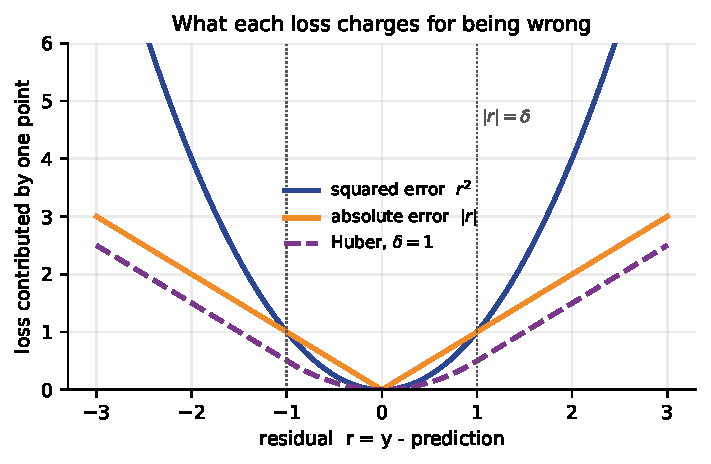
\includegraphics[width=0.82\textwidth]{losscurves.pdf}
  \caption{What each loss charges for a single residual. The squared error is a
  bowl; the absolute error is a V with a kink at zero; Huber is the bowl near
  zero and the V far away.}
  \label{fig:losscurves}
\end{figure}

\subsection{The result that matters: MSE fits the mean, MAE fits the median}
\label{sec:meanmedian}

Here is the cleanest way to see the difference. Forget features entirely and
ask the simplest question in statistics: \emph{if I must predict one constant
$c$ for every observation, what constant should I choose?}

The answer depends entirely on the loss:

\begin{itemize}[leftmargin=*]
  \item Minimising $\sum (y_i - c)^2$ gives $c = \bar{y}$, the \textbf{mean}.
  \item Minimising $\sum \lvert y_i - c\rvert$ gives $c = \mathrm{median}(y)$.
\end{itemize}

Both are worth proving to yourself; the first is one line of calculus, the
second a counting argument (Question~\ref{q:median}).

Now the consequence. Take six observations, and drag one of them far away.

\begin{lstlisting}
clean   = np.array([10., 11., 12., 13., 14., 14.])
outlier = np.array([10., 11., 12., 13., 14., 94.])

for name, d in [("clean", clean), ("with outlier", outlier)]:
    print("%-13s mean=%.4f  median=%.4f" % (name, d.mean(), np.median(d)))
\end{lstlisting}
\begin{codeout}
clean         mean=12.3333  median=12.5000
with outlier  mean=25.6667  median=12.5000
\end{codeout}

One corrupted reading moved the MSE-optimal prediction from $12.33$ to
$\mathbf{25.67}$ --- past every single clean observation. The MAE-optimal
prediction did not move at all.

We can confirm that these really are the minimisers rather than taking it on
faith, by evaluating both losses on a fine grid of candidate constants:

\begin{lstlisting}
grid = np.linspace(0, 100, 200001)
mse_curve = ((outlier[:, None] - grid[None, :])**2).mean(axis=0)
mae_curve = (np.abs(outlier[:, None] - grid[None, :])).mean(axis=0)
print("argmin MSE ->", round(grid[mse_curve.argmin()], 4), " mean   =", outlier.mean())
print("argmin MAE ->", round(grid[mae_curve.argmin()], 4), " median =", np.median(outlier))
\end{lstlisting}
\begin{codeout}
argmin MSE -> 25.6665  mean   = 25.666666666666668
argmin MAE -> 12.0  median = 12.5
\end{codeout}

\begin{caution}[Why the MAE grid search returned 12.0 and not 12.5]
This is not a bug, and it is worth understanding. With an \emph{even} number of
observations the absolute-error loss is not minimised at a single point --- it
is flat across the whole interval between the two central observations, here
$[12, 13]$. Every constant in that interval gives exactly the same MAE.

\texttt{argmin} returns the \emph{first} index achieving the minimum, so it
reports the left end, $12.0$. NumPy's \texttt{median} conventionally returns the
midpoint, $12.5$. Both are correct minimisers; neither is more right than the
other.

The flat region is also why MAE is harder to optimise than MSE: a flat loss
gives a zero gradient, and an optimiser standing on a plateau does not know
which way to go.
\end{caution}

\begin{figure}[htbp]
  \centering
  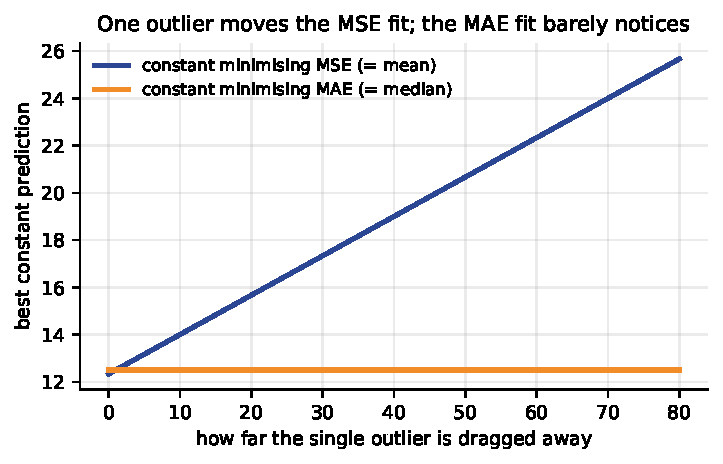
\includegraphics[width=0.82\textwidth]{outlier.pdf}
  \caption{The best constant prediction as a single outlier is dragged further
  and further away. The MSE solution follows it without limit; the MAE solution
  is unmoved.}
  \label{fig:outlier}
\end{figure}

\begin{keyidea}[The sentence to remember]
Choosing a loss is not choosing how to \emph{score} your model. It is choosing
\emph{what your model will become}. MSE builds a model of the average case; MAE
builds a model of the typical case. On clean symmetric data they nearly agree.
On data with a heavy tail they answer different questions.
\end{keyidea}

\subsection{Huber loss}

We would like MSE's smooth, well-behaved gradient near zero and MAE's
indifference to outliers far from zero. Huber loss simply uses each where it is
wanted:

\[
  L_\delta(r) \;=\;
  \begin{cases}
    \tfrac{1}{2} r^2, & \lvert r\rvert \le \delta,\\[4pt]
    \delta\left(\lvert r\rvert - \tfrac{1}{2}\delta\right), & \lvert r\rvert > \delta .
  \end{cases}
\]

The second branch is exactly the tangent line to the first at $r = \delta$, so
the two pieces meet with matching value \emph{and} matching slope. The result
is differentiable everywhere, including at the join.

\begin{worked}[Huber by hand, with delta equal to one]
Same four residuals as before: $0.5,\ -0.5,\ -2.0,\ 1.0$.

\begin{itemize}[leftmargin=*]
  \item $\lvert 0.5\rvert \le 1$, so quadratic: $\tfrac12 (0.5)^2 = 0.125$.
  \item $\lvert -0.5\rvert \le 1$, so quadratic: $0.125$.
  \item $\lvert -2.0\rvert > 1$, so linear: $1\cdot(2 - 0.5) = 1.5$.
  \item $\lvert 1.0\rvert \le 1$, so quadratic: $\tfrac12 (1)^2 = 0.5$.
\end{itemize}

Mean $= (0.125+0.125+1.5+0.5)/4 = 2.25/4 = \mathbf{0.5625}$.

Compare with the squared error, where that third point alone contributed $4.0$.
Huber charged it $1.5$.
\end{worked}

\begin{lstlisting}
def huber(r, d=1.0):
    a = np.abs(r)
    return np.where(a <= d, 0.5*r**2, d*(a - 0.5*d))

print("per point ", huber(r, 1.0))
print("mean      ", huber(r, 1.0).mean())
\end{lstlisting}
\begin{codeout}
per point  [0.125 0.125 1.5   0.5  ]
mean       0.5625
\end{codeout}

\begin{figure}[htbp]
  \centering
  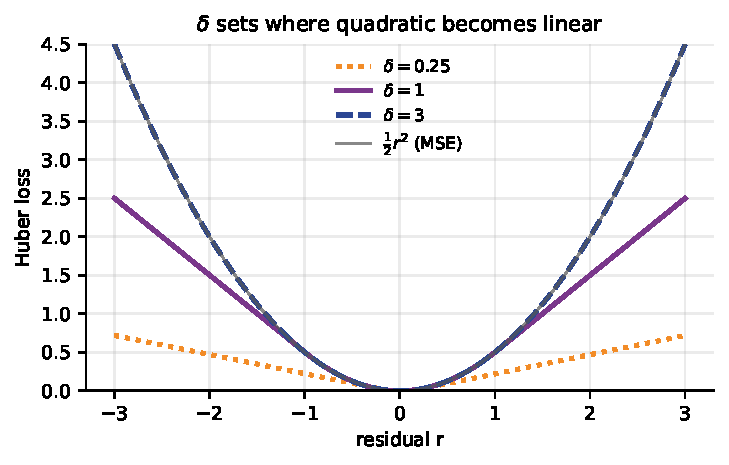
\includegraphics[width=0.82\textwidth]{huberdelta.pdf}
  \caption{$\delta$ controls where the loss stops being quadratic. Small
  $\delta$ behaves almost like MAE; large $\delta$ is almost pure MSE over the
  range shown.}
  \label{fig:huberdelta}
\end{figure}

\begin{caution}[$\delta$ is a hyperparameter with units]
$\delta$ is measured in the units of $y$. A $\delta$ of $1$ means something
completely different for house prices in lakhs than for temperatures in
degrees. Choose it by cross-validation, or set it from a robust scale estimate
of the residuals --- never copy it from a tutorial.
\end{caution}

\begin{tryit}
Re-run the constant-prediction experiment from Section~\ref{sec:meanmedian}
using Huber loss with $\delta = 1$ and again with $\delta = 50$, and find the
minimising constant on a grid. You should find the $\delta=1$ answer sits near
the median and the $\delta=50$ answer near the mean, because when $\delta$ is
larger than every residual Huber \emph{is} scaled MSE.
\end{tryit}

\newpage
% =========================================================================
\section{Classification losses}
\label{sec:clf}

Now the prediction is a class. The obvious loss is: charge $1$ for a wrong
answer and $0$ for a right one. This is the \textbf{0--1 loss}, and it is
exactly what accuracy measures.

It is also almost useless for training.

\subsection{Why accuracy cannot be the loss}

Consider a one-parameter classifier that predicts class $1$ when $wx > 0$. Vary
$w$ and watch both accuracy and cross-entropy:

\begin{lstlisting}
X = np.array([[1.0], [2.0], [-1.0], [-2.0]])
y = np.array([1, 1, 0, 0])

for w in [-2.0, -1.0, 0.0, 1.0, 2.0]:
    z = X.ravel() * w
    acc = ((z > 0).astype(int) == y).mean()
    p = 1 / (1 + np.exp(-z))
    ll = -np.mean(y*np.log(p+1e-12) + (1-y)*np.log(1-p+1e-12))
    print("w=%5.1f  accuracy=%.2f  log-loss=%.4f" % (w, acc, ll))
\end{lstlisting}
\begin{codeout}
w= -2.0  accuracy=0.00  log-loss=3.0725
w= -1.0  accuracy=0.00  log-loss=1.7201
w=  0.0  accuracy=0.50  log-loss=0.6931
w=  1.0  accuracy=1.00  log-loss=0.2201
w=  2.0  accuracy=1.00  log-loss=0.0725
\end{codeout}

Look at the two columns.

Accuracy takes three values in total: $0$, $0.5$, $1$. It is a step function ---
flat almost everywhere, with sudden jumps. Its derivative is zero wherever it
is defined, so gradient descent standing anywhere on it receives the message
``every direction is equally good''. And accuracy cannot distinguish $w=1$ from
$w=2$ at all, though the second is clearly a more confident fit.

Cross-entropy decreases smoothly and strictly the whole way. Every value of $w$
gets a gradient telling it which way to move and by how much.

\begin{keyidea}[Surrogate losses]
We optimise a \textbf{surrogate}: a smooth loss that is a good stand-in for the
thing we actually care about. Cross-entropy and hinge are the two standard
surrogates for the 0--1 loss. This is why the number you optimise and the
number you report are so often different --- not carelessness, but necessity.
\end{keyidea}

\subsection{Binary cross-entropy}

The model outputs $p_i$, its claimed probability that example $i$ belongs to
class $1$. With true label $y_i \in \{0,1\}$:

\[
  \mathrm{BCE} \;=\; -\frac{1}{n}\sum_{i=1}^{n}
    \Big[\, y_i \log p_i \;+\; (1-y_i)\log(1-p_i) \,\Big]
\]

The bracket looks like two terms but only ever contributes one: when $y_i=1$
the second term vanishes, and when $y_i=0$ the first does. So the formula says
something very simple:

\begin{keyidea}
Take the probability the model assigned to \emph{the class that was actually
correct}. Take its negative logarithm. Average over the data. That is all
cross-entropy is.
\end{keyidea}

\begin{worked}[Binary cross-entropy by hand]
Three emails. $y=1$ means spam. The model reports $p$, its probability of spam.

\begin{center}
\begin{tabular}{@{}lrrr@{}}
\toprule
true $y$              & 1   & 0   & 1\\
model $p$ (spam)      & 0.9 & 0.2 & 0.4\\
\midrule
prob.\ of correct class & 0.9 & 0.8 & 0.4\\
$-\log(\cdot)$          & 0.1054 & 0.2231 & 0.9163\\
\bottomrule
\end{tabular}
\end{center}

Row three is the only step with any content: for the first and third emails the
correct class was spam, so we take $p$; for the second the correct class was
not-spam, so we take $1-p = 0.8$.

\[
  \mathrm{BCE} = \frac{0.1054 + 0.2231 + 0.9163}{3} = \mathbf{0.4149}
\]

The third email dominates. The model was not confidently wrong there --- it said
$0.4$ for something that was spam, a near coin-flip --- and it still cost more
than the other two combined.
\end{worked}

\begin{lstlisting}
from sklearn.metrics import log_loss

y = np.array([1, 0, 1])
p = np.array([0.9, 0.2, 0.4])
pc = np.where(y == 1, p, 1 - p)         # prob assigned to the correct class

print("prob of correct", pc)
print("-log each      ", -np.log(pc))
print("BCE by hand    ", (-np.log(pc)).mean())
print("BCE sklearn    ", log_loss(y, p))
\end{lstlisting}
\begin{codeout}
prob of correct [0.9 0.8 0.4]
-log each       [0.1054 0.2231 0.9163]
BCE by hand     0.414931599615397
BCE sklearn     0.414931599615397
\end{codeout}

\subsection{Confident and wrong}

The logarithm is what gives cross-entropy its character:

\begin{center}
\begin{tabular}{@{}rrl@{}}
\toprule
$p$ on correct class & loss & \\
\midrule
0.99  & 0.0101 & confident and right --- nearly free\\
0.90  & 0.1054 & \\
0.50  & 0.6931 & a coin flip costs $\log 2$\\
0.10  & 2.3026 & \\
0.01  & 4.6052 & confident and wrong --- 458$\times$ the cost of being right\\
0.001 & 6.9078 & and it keeps going\\
\bottomrule
\end{tabular}
\end{center}

As $p \to 0$ the loss grows without bound. A model that is certain and wrong on
even one training example pays an enormous price, which is precisely the
behaviour we want: it forces models to be honest about their uncertainty rather
than confidently guessing.

\begin{figure}[htbp]
  \centering
  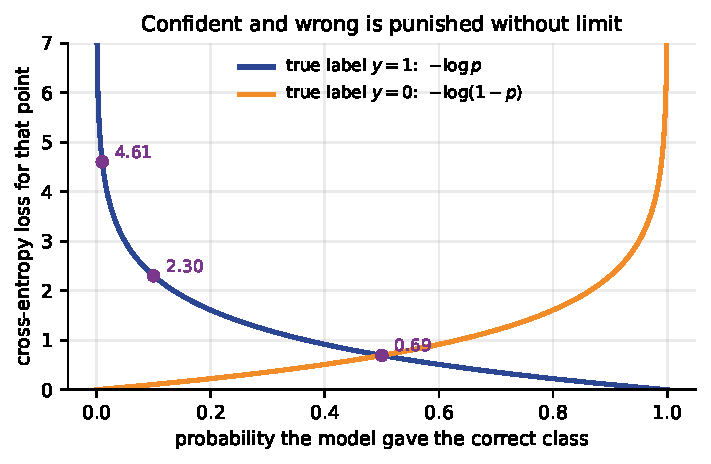
\includegraphics[width=0.82\textwidth]{logloss.pdf}
  \caption{Cross-entropy against the probability given to the correct class.
  Being right is cheap; being confidently wrong is unboundedly expensive.}
  \label{fig:logloss}
\end{figure}

\begin{caution}[$\log 0$ is not a number]
A model that outputs exactly $0$ or exactly $1$ produces an infinite loss and
your training run dies. Every library therefore clips probabilities into
$[\varepsilon,\, 1-\varepsilon]$. This is why you should feed
\texttt{log\_loss} probabilities rather than hard $0/1$ predictions --- and why
you should never write your own cross-entropy without an $\varepsilon$, as in
the \texttt{+1e-12} above.
\end{caution}

\subsection{Categorical and sparse categorical cross-entropy}

With $K$ classes the model outputs a probability vector $\mathbf{p}_i$ summing
to one. The loss is unchanged in spirit:

\[
  \mathrm{CCE} \;=\; -\frac{1}{n}\sum_{i=1}^{n}\sum_{k=1}^{K}
     y_{ik} \log p_{ik}
\]

where $y_{ik}$ is $1$ if example $i$ is of class $k$ and $0$ otherwise. Because
only one $y_{ik}$ per row is non-zero, the inner sum again picks out a single
term: the log-probability of the correct class.

\textbf{Categorical} and \textbf{sparse categorical} cross-entropy are
\emph{the same loss}. They differ only in how you hand over the labels:

\begin{center}
\begin{tabular}{@{}lll@{}}
\toprule
& \textbf{Label format} & \textbf{Example for 3 classes}\\
\midrule
Categorical        & one-hot rows          & \texttt{[[1,0,0],[0,1,0],[0,0,1]]}\\
Sparse categorical & integer class indices & \texttt{[0, 1, 2]}\\
\bottomrule
\end{tabular}
\end{center}

\begin{lstlisting}
P = np.array([[0.7, 0.2, 0.1],
              [0.1, 0.8, 0.1],
              [0.2, 0.2, 0.6]])
onehot = np.array([[1,0,0], [0,1,0], [0,0,1]])
sparse = np.array([0, 1, 2])

print("categorical", -np.sum(onehot * np.log(P), axis=1).mean())
print("sparse     ", -np.log(P[np.arange(3), sparse]).mean())
print("sklearn    ", log_loss(sparse, P))
\end{lstlisting}
\begin{codeout}
categorical 0.3635480396729776
sparse      0.3635480396729776
sklearn     0.3635480396729776
\end{codeout}

Identical to sixteen decimal places, because it is the same arithmetic.

\begin{caution}[Why the sparse form exists]
It is purely a memory and speed optimisation. With $K = 10{,}000$ classes --- a
language model's vocabulary, say --- the one-hot matrix for a batch of $256$
examples holds $2.56$ million numbers of which $256$ are non-zero. The sparse
form stores $256$ integers and indexes directly. Same loss, same gradients, a
fraction of the memory.

Choosing the wrong one is one of the most common beginner errors in Keras and
PyTorch, and the error message is rarely helpful. Look at the shape of your
labels: 2-D means categorical, 1-D means sparse.
\end{caution}

\newpage
% =========================================================================
\section{Margin losses}
\label{sec:margin}

Cross-entropy needs a probability. Some classifiers do not produce one --- a
support vector machine outputs a raw score $f(x)$, positive for one class and
negative for the other. For these we use \textbf{margin} losses.

Relabel the classes as $y \in \{-1, +1\}$ and define the \textbf{margin}
\[
  m_i \;=\; y_i \, f(x_i) .
\]

The margin is positive exactly when the prediction is correct, and its
magnitude says how decisively. This single number is all a margin loss looks at.

\subsection{Hinge loss}

\[
  L_{\mathrm{hinge}}(m) \;=\; \max(0,\; 1 - m)
\]

Read it directly: if the margin is at least $1$, the loss is zero. Otherwise
you pay the shortfall.

\begin{keyidea}
Hinge loss stops caring once you are right by a comfortable margin. Cross-entropy
never entirely stops caring --- it will always take a little more confidence if
it can get it. That difference is why SVMs are determined by a handful of
support vectors while logistic regression is influenced by every point.
\end{keyidea}

\begin{worked}[Hinge loss by hand]
Three points, true labels in $\{-1,+1\}$, raw scores $f$.

\begin{center}
\begin{tabular}{@{}lrrr@{}}
\toprule
true $y$        & $+1$ & $-1$ & $+1$\\
score $f(x)$    & 2.0  & $-0.5$ & 0.3\\
\midrule
margin $m=yf$   & 2.0  & 0.5  & 0.3\\
$\max(0, 1-m)$  & 0.0  & 0.5  & 0.7\\
\bottomrule
\end{tabular}
\end{center}

\[
  L = \frac{0.0 + 0.5 + 0.7}{3} = \frac{1.2}{3} = \mathbf{0.4}
\]

Every one of these three points is classified \emph{correctly} --- all three
margins are positive. Yet two of them still incur a loss, because they sit
inside the margin band. This is the behaviour that produces a wide separating
boundary rather than one that merely separates.
\end{worked}

\begin{lstlisting}
from sklearn.metrics import hinge_loss

ys = np.array([1, -1, 1])
f  = np.array([2.0, -0.5, 0.3])
m  = ys * f

print("margins      ", m)
print("hinge each   ", np.maximum(0, 1 - m))
print("hinge by hand", np.maximum(0, 1 - m).mean())
print("hinge sklearn", hinge_loss(ys, f))
\end{lstlisting}
\begin{codeout}
margins       [2.  0.5 0.3]
hinge each    [0.  0.5 0.7]
hinge by hand 0.39999999999999997
hinge sklearn 0.39999999999999997
\end{codeout}

\begin{caution}
That is $0.4$, printed as \texttt{0.39999999999999997}. Binary floating point
cannot represent $0.4$ exactly. Never test loss values with \texttt{==}; use
\texttt{np.isclose} or \texttt{math.isclose}.
\end{caution}

\subsection{Squared hinge, and the family portrait}

Squaring the hinge, $\max(0, 1-m)^2$, gives a smooth loss (no kink at $m=1$)
that punishes large violations harder. It is more sensitive to outliers than
plain hinge, for exactly the reason MSE is more sensitive than MAE.

\begin{figure}[htbp]
  \centering
  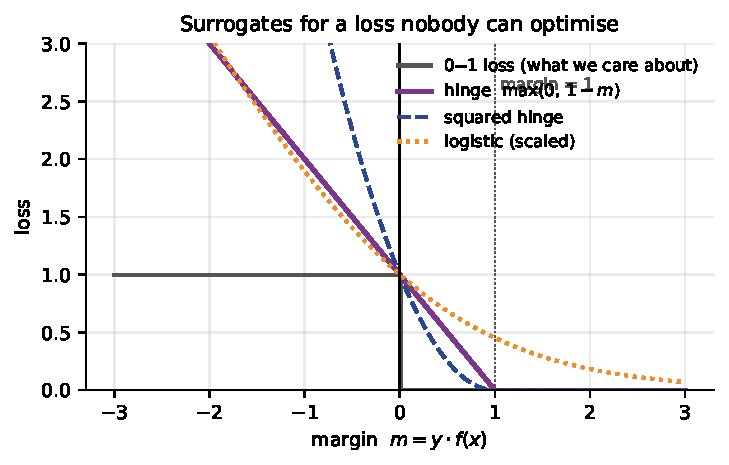
\includegraphics[width=0.82\textwidth]{margin.pdf}
  \caption{The 0--1 loss we would like to minimise, and the three smooth
  surrogates that we minimise instead. All three are upper bounds on the 0--1
  loss, which is what makes them legitimate stand-ins.}
  \label{fig:margin}
\end{figure}

Read Figure~\ref{fig:margin} carefully; it is the summary of this whole
section.

\begin{itemize}[leftmargin=*]
  \item The grey step is what we care about: wrong ($m \le 0$) costs $1$, right
    costs $0$.
  \item Each smooth curve sits \emph{above} the step everywhere. Driving the
    surrogate down therefore drives the 0--1 loss down too.
  \item Hinge reaches exactly zero at $m=1$ and stays there. Logistic
    approaches zero but never arrives.
  \item For very negative margins, hinge grows linearly and squared hinge
    quadratically --- so one badly mislabelled point disturbs a squared-hinge
    model far more.
\end{itemize}

\subsection{Triplet loss}

The last loss in this lecture answers a different question. Sometimes we do not
want to classify at all --- we want to \emph{learn a representation} in which
similar things are close together. Face recognition is the standard example:
you cannot train a classifier with one output per person when new people keep
arriving.

Triplet loss works on three examples at a time:

\begin{itemize}[leftmargin=*]
  \item an \textbf{anchor} $a$,
  \item a \textbf{positive} $p$ --- same identity as the anchor,
  \item a \textbf{negative} $n$ --- a different identity.
\end{itemize}

\[
  L \;=\; \max\Big(0,\; d(a,p) \;-\; d(a,n) \;+\; \alpha\Big)
\]

In words: the anchor should be closer to the positive than to the negative, by
at least a margin $\alpha$. If it already is, the loss is zero and nothing is
learned from this triplet.

\begin{figure}[htbp]
  \centering
  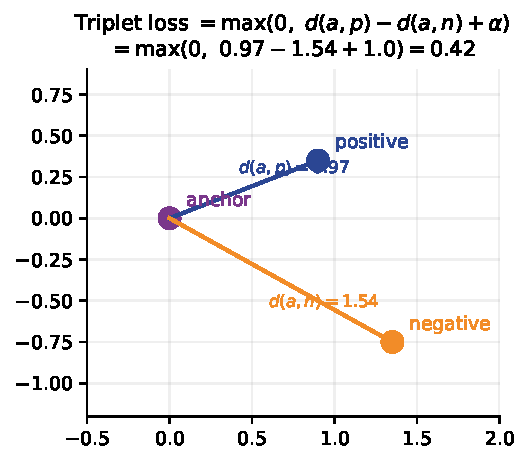
\includegraphics[width=0.68\textwidth]{triplet.pdf}
  \caption{A triplet that still has something to teach. The anchor is closer to
  the positive than to the negative, but not by the required margin, so the
  loss is non-zero and the embedding will be adjusted.}
  \label{fig:triplet}
\end{figure}

For the configuration in Figure~\ref{fig:triplet}, with $\alpha = 1$:

\[
  L = \max\big(0,\; 0.97 - 1.54 + 1.0\big) = \mathbf{0.42}
\]

The ordering is already correct --- the positive is nearer --- but only by
$0.58$, short of the margin of $1$, so a penalty remains.

\begin{caution}[Most triplets teach you nothing]
Pick three examples at random and the constraint is usually already satisfied,
giving zero loss and zero gradient. Practical systems therefore spend most of
their engineering effort on \emph{triplet mining}: actively searching for the
hard cases where $d(a,p)$ is nearly as large as $d(a,n)$. Without mining,
training stalls almost immediately.
\end{caution}

\newpage
% =========================================================================
\section{Choosing a loss}
\label{sec:choose}

\begin{center}
\begin{tabular}{@{}p{4.6cm}p{3.1cm}p{6.4cm}@{}}
\toprule
\textbf{Situation} & \textbf{Use} & \textbf{Because}\\
\midrule
Regression, clean data, errors roughly symmetric & MSE & Smooth, fast, and the mean is the sensible target\\[3pt]
Regression, outliers you do not trust & MAE & Fits the typical case; one bad reading cannot drag it\\[3pt]
Regression, outliers you cannot exclude but must not dominate & Huber & Quadratic where it matters, linear where it would distort\\[3pt]
Two classes, want probabilities & Binary cross-entropy & Calibrated outputs; punishes confident errors\\[3pt]
$K$ classes, labels one-hot & Categorical cross-entropy & Same loss, one-hot API\\[3pt]
$K$ classes, labels are integers & Sparse categorical cross-entropy & Same loss, far less memory\\[3pt]
Two classes, want a wide boundary, no probabilities needed & Hinge & Ignores points already safely correct\\[3pt]
Learning an embedding where "similar" must mean "close" & Triplet & Trains on relative distance, handles unseen identities\\
\bottomrule
\end{tabular}
\end{center}

\begin{caution}[Do not choose by asking which gives the smaller number]
Losses are on different scales and are not comparable to each other. An MAE of
$1.0$ is not "better" than an MSE of $1.375$ --- they are different quantities
in different units, computed from the identical predictions, as the worked
example in Section~\ref{sec:reg} shows.

Compare \emph{models} using a single fixed metric on held-out data. Use the
loss to train; use the metric to decide.
\end{caution}

% =========================================================================
\section{Summary}

\begin{enumerate}[leftmargin=*]
  \item A loss compresses a set of mistakes into one number, and that choice
    declares what kind of mistake you consider serious.
  \item Loss, cost and metric are three different things. Loss and metric are
    allowed to differ, and often must.
  \item MSE fits the mean; MAE fits the median. One outlier moved our
    MSE-optimal constant from $12.33$ to $25.67$ and left the MAE-optimal
    constant untouched.
  \item Huber is MSE near zero and MAE far away, joined smoothly at $\delta$.
    $\delta$ carries the units of $y$.
  \item Accuracy cannot be a training loss: it is a step function with zero
    gradient. We minimise smooth surrogates instead.
  \item Cross-entropy is the negative log of the probability given to the
    correct class. Confident and wrong is unboundedly expensive.
  \item Categorical and sparse categorical cross-entropy are the same loss with
    different label formats.
  \item Hinge loss charges nothing once the margin exceeds $1$, which is what
    produces a wide margin and a small set of support vectors.
  \item Triplet loss trains representations by relative distance, and needs
    hard-triplet mining to make progress.
\end{enumerate}

\newpage
% =========================================================================
\section{Practice questions}

Attempt these before reading Section~\ref{sec:solutions}.

\begin{enumerate}[leftmargin=*]
  \item Predictions $\hat y = [4, 7, 10]$ for true values $y = [5, 5, 5]$.
    Compute MSE, MAE and RMSE by hand.

  \item\label{q:median} Prove that the constant $c$ minimising
    $\sum_i \lvert y_i - c\rvert$ is a median of the $y_i$.
    \emph{Hint:} think about how the total changes as $c$ moves slightly right.

  \item A model predicts probability $0.7$ for the correct class on every one
    of $50$ examples. What is the cross-entropy? Now one example changes to
    $0.001$ on the correct class. What is the new value?

  \item You are predicting delivery times. Being $10$ minutes late is more than
    twice as bad as being $5$ minutes late for your users, and occasional
    sensor glitches produce impossible readings. Which loss, and why?

  \item For $y=+1$ and score $f(x) = 3$, give the hinge loss and the logistic
    loss. Which is exactly zero, and what does that imply about whether this
    point affects training?

  \item Huber with $\delta = 100$ is applied to residuals that never exceed
    $10$. What loss have you effectively chosen? What does this tell you about
    setting $\delta$ without looking at your data?

  \item A classmate reports "my model achieved a loss of $0.31$, which beats the
    published baseline of $0.44$." Give two distinct reasons this comparison
    may be meaningless.

  \item Your labels are the integers $[2, 0, 1]$ and your model outputs a
    $3\times 3$ matrix of probabilities. Which cross-entropy variant do you
    use, and what breaks if you choose the other one?

  \item For a triplet with $d(a,p) = 0.4$, $d(a,n) = 1.9$ and $\alpha = 1$,
    compute the loss. What does your answer imply about how much this triplet
    contributes to training?

  \item MSE is minimised by the mean and MAE by the median. What summary
    statistic is minimised by the 0--1 loss, if we apply it to a discrete
    prediction problem? Justify your answer.
\end{enumerate}

\newpage
% =========================================================================
\section{Solutions}
\label{sec:solutions}

\textbf{1.} Residuals $r = y - \hat y = [1, -2, -5]$.
$\mathrm{MSE} = (1 + 4 + 25)/3 = 30/3 = 10$.
$\mathrm{MAE} = (1 + 2 + 5)/3 = 8/3 = 2.667$.
$\mathrm{RMSE} = \sqrt{10} = 3.162$.
Note RMSE $>$ MAE, which is always true and is a direct consequence of squaring
inflating the largest residual.

\medskip
\textbf{2.} Order the observations. Suppose $c$ sits so that $k$ observations
lie strictly below it and $n-k$ strictly above. Move $c$ right by a small
$\epsilon$ (small enough to cross no observation). Each of the $k$ points below
becomes $\epsilon$ further away; each of the $n-k$ above becomes $\epsilon$
nearer. The total changes by $\epsilon\,\big(k - (n-k)\big) = \epsilon(2k-n)$.

This is negative while $k < n/2$, so moving right helps; positive once
$k > n/2$, so moving right hurts. The minimum is therefore where $k = n/2$ ---
a median. When $n$ is even any point between the two central observations gives
$2k - n = 0$, so the whole interval is optimal, which is exactly the plateau we
observed numerically in Section~\ref{sec:meanmedian}.

\medskip
\textbf{3.} All fifty at $0.7$: the loss is just $-\log 0.7 = 0.3567$ (the mean
of identical values). Changing one to $0.001$:
\[
  \frac{49 \times 0.3567 + 6.9078}{50}
  = \frac{17.477 + 6.908}{50} = 0.4877 .
\]
A single confidently wrong example raised the loss by $37\%$. That sensitivity
is the design intent, but it also means one mislabelled training row can
noticeably distort your objective --- a reason to inspect the highest-loss
examples after training.

\medskip
\textbf{4.} The two requirements conflict, which is the point of the question.
"More than twice as bad" argues for a super-linear penalty, i.e.\ MSE.
"Impossible sensor readings" argues against MSE, which those readings would
dominate. \textbf{Huber} resolves it: quadratic over the range of genuine
lateness, linear beyond, with $\delta$ set at the boundary of physically
plausible delays. Cleaning the impossible readings first is better still ---
choosing a robust loss is not a substitute for fixing your data.

\medskip
\textbf{5.} Margin $m = yf(x) = 3$. Hinge $= \max(0, 1-3) = 0$. Logistic
$= \log(1 + e^{-3}) = 0.0486$. The hinge loss is exactly zero, so this point
contributes no gradient and could be deleted from the training set without
changing the SVM at all --- it is not a support vector. Under logistic loss it
still contributes a small pull, so it is never entirely irrelevant.

\medskip
\textbf{6.} With $\delta = 100$ and $\lvert r\rvert \le 10$ always, the
condition $\lvert r\rvert \le \delta$ holds for every point, so only the
quadratic branch is ever used. You have chosen $\tfrac12 \times$ MSE, and gained
none of Huber's robustness while adding a hyperparameter. The lesson: $\delta$
must sit inside the range your residuals actually occupy, so it has to be set
after looking at the residual distribution.

\medskip
\textbf{7.} Any two of: (i) the two numbers may be different losses entirely ---
$0.31$ MAE against $0.44$ MSE compares nothing; (ii) they may be computed on
different datasets, or different train/test splits; (iii) one may be a training
loss and the other a test loss; (iv) the target variable may be scaled
differently, and every regression loss inherits the units of $y$; (v) with a
different class balance, cross-entropy values are not comparable.

\medskip
\textbf{8.} Labels are 1-D integers, so use \textbf{sparse categorical
cross-entropy}. If you pass integer labels to the categorical form, the library
will either raise a shape error (expecting $n \times K$, receiving $n$) or, in
the worst case, silently broadcast and compute a meaningless number. This is
why you check label shape before choosing, rather than after debugging.

\medskip
\textbf{9.} $L = \max(0,\; 0.4 - 1.9 + 1) = \max(0, -0.5) = \mathbf{0}$. The
constraint is already satisfied with room to spare, so the gradient is zero and
this triplet contributes \emph{nothing} to training. It is exactly the kind of
easy triplet that mining exists to avoid.

\medskip
\textbf{10.} The \textbf{mode}. The 0--1 loss charges $1$ for every prediction
that is not exactly right, so the expected loss of predicting class $c$ is
$1 - P(Y = c)$, minimised by choosing the most probable class. This completes a
pleasing pattern: squared error gives the mean, absolute error the median,
0--1 error the mode --- the three classical measures of central tendency each
fall out of a different loss.

\newpage
% =========================================================================
\section{References and further reading}

All links were checked on 5 August 2026. Free resources are marked
\textbf{[free]}.

\subsection*{Textbooks}

\begin{itemize}[leftmargin=*]
  \item Bishop, \emph{Pattern Recognition and Machine Learning}, Springer 2006.
    \S1.5 (decision theory and loss), \S4.3 (logistic regression and
    cross-entropy), \S7.1 (maximum margin and hinge). A free PDF is hosted by
    Microsoft Research; their site blocks automated link checks, so no direct
    URL is printed here --- search for the title plus ``Microsoft Research''.
  \item M\"uller and Guido, \emph{Introduction to Machine Learning with Python},
    O'Reilly 2016. Chapter 2 for where these losses sit inside the estimators
    you will actually call.
  \item Shalev-Shwartz and Ben-David, \emph{Understanding Machine Learning:
    From Theory to Algorithms}, Cambridge 2014. \textbf{[free]} Chapter 15 on
    surrogate losses and why upper-bounding the 0--1 loss is the right move.
    \url{https://www.cs.huji.ac.il/~shais/UnderstandingMachineLearning/}
  \item Murphy, \emph{Probabilistic Machine Learning: An Introduction},
    MIT Press 2022. \textbf{[free]} Chapter 5 for the decision-theoretic view.
    \url{https://probml.github.io/pml-book/book1.html}
\end{itemize}

\subsection*{Online courses}

\begin{itemize}[leftmargin=*]
  \item \textbf{NPTEL, Introduction to Machine Learning} --- Prof.\ Balaraman
    Ravindran, IIT Madras. The closest match to this syllabus.
    \textbf{[free]} \url{https://nptel.ac.in/courses/106106139}
  \item \textbf{SWAYAM} --- national portal hosting NPTEL and other Indian
    university courses. \textbf{[free]} \url{https://swayam.gov.in/}
  \item \textbf{Google Machine Learning Crash Course} --- the "Descending into
    ML" and "Logistic Regression" modules cover squared loss and log loss with
    interactive exercises. \textbf{[free]}
    \url{https://developers.google.com/machine-learning/crash-course}
\end{itemize}

\subsection*{Videos}

\begin{itemize}[leftmargin=*]
  \item StatQuest, \emph{Entropy (for data science) Clearly Explained}. Builds
    the logarithm in cross-entropy from first principles.
    \textbf{[free]} \url{https://youtu.be/YtebGVx-Fxw}
  \item StatQuest, \emph{Support Vector Machines Part 1 (of 3): Main Ideas}.
    Where the margin comes from and why points beyond it stop mattering.
    \textbf{[free]} \url{https://youtu.be/efR1C6CvhmE}
  \item StatQuest video index --- short, clear explanations for most topics in
    this syllabus. \textbf{[free]} \url{https://statquest.org/video-index/}
\end{itemize}

\subsection*{Documentation}

\begin{itemize}[leftmargin=*]
  \item scikit-learn, \emph{Metrics and scoring}. The catalogue of losses and
    metrics, and the scorer interface. \textbf{[free]}
    \url{https://scikit-learn.org/stable/modules/model_evaluation.html}
  \item scikit-learn, \emph{Common pitfalls and recommended practices}.
    \textbf{[free]}
    \url{https://scikit-learn.org/stable/common_pitfalls.html}
  \item \emph{Dive into Deep Learning}, \S3.4 (softmax regression and
    cross-entropy). Runnable, with the derivations laid out.
    \textbf{[free]} \url{https://d2l.ai/chapter_linear-classification/softmax-regression.html}
\end{itemize}

\subsection*{Articles}

\begin{itemize}[leftmargin=*]
  \item Huber, ``Robust Estimation of a Location Parameter'', \emph{Annals of
    Mathematical Statistics} 35(1), 1964. The original paper; the first two
    pages are readable and set up exactly the mean-versus-median tension in
    Section~\ref{sec:meanmedian}.
  \item Schroff, Kalenichenko and Philbin, ``FaceNet: A Unified Embedding for
    Face Recognition and Clustering'', CVPR 2015. Where triplet loss and
    triplet mining were popularised. \textbf{[free]}
    \url{https://arxiv.org/abs/1503.03832}
\end{itemize}

\notesources{\AMLUnitIISources}

\end{document}
